\documentclass[twoside,twocolumn]{article}
    \usepackage[a4paper, left=2cm, right=2cm]{geometry} % A4 paper size and thin margins
    \usepackage[sc]{mathpazo} % Use the Palatino font
    \usepackage[T1]{fontenc} % Use 8-bit encoding that has 256 glyphs
    \usepackage{microtype} % Slightly tweak font spacing for aesthetics
    \usepackage[english]{babel} % Language hyphenation and typographical rules
    \usepackage{booktabs} % Horizontal rules in tables
    \usepackage{enumitem} % Customized lists
    \usepackage[table,xcdraw]{xcolor}
    \usepackage[utf8]{inputenc} % Required for inputting international characters
    \usepackage{parskip}
    \usepackage{graphicx}
    \usepackage{hyperref}
    \usepackage{pdfpages}
    \usepackage{amsmath}
    \usepackage{esvect}
    \usepackage{listings}
    \usepackage[title]{appendix}
    \hypersetup{
        colorlinks=true,
        linkcolor=blue,
        filecolor=magenta,      
        urlcolor=cyan,
    }
    \urlstyle{same}
    \setlength{\parindent}{18pt}
    \setlist[itemize]{noitemsep} % Make itemize lists more compact
    \makeatletter
    \newcommand*{\rom}[1]{\expandafter\@slowromancap\romannumeral #1@}
    \g@addto@macro{\UrlBreaks}{\UrlOrds}
    \makeatother

    \title{\LARGE \bf
    Music Genre Identification
    }
    
    \author{ \parbox{3 in}{\centering Chongyi Xu \\
             University of Washington\\
             AMATH 482/582 Winter Quarter 2018\\
             {\tt\small chongyix@uw.edu}}
    }

    \begin{document}
    \maketitle

    %----------------------------------------------------------------------------------------
    %	ARTICLE CONTENTS
    %----------------------------------------------------------------------------------------
    \begin{abstract}

    For this project, we are focusing on using machine learning techniques to classify
    different music bands/genres. There are generally two techniques to be used in this project - 
    Naive Bayes, and Decision Trees.
        
    \end{abstract}

    \linespread{1.05} % Line spacing - Palatino needs more space between lines
    %------------------------------------------------
    \section{Introduction and Overview}
    \subsection{Introudction}
    Humans classify audio signals all the time without paying attentions. Classifying who is speaking in a group, or 
    realizing the person on the other side of the phone call, or classifying whether the music that is playing on the 
    radio is rock or jazz. But the problem comes that how could we tell machine to know that, who is speaking (cocktail
    party problem), or what genre does the playing music belong to.

    %------------------------------------------------
    \subsection{Overview}
    The project has three tests to be completed.
    \begin{itemize}
        \item Band Classification
        \item The Case for Seattle
        \item Genre Classification
    \end{itemize}
    I will pick 6 songs for each of Michael Jackson, Soundgarden, and Beethoven for the Band Classification Test.
    For the Seattle Case Test, I will pick Soundgarden, Alice in Chains, and Pearl Jam to classify 5-sound sound clips with 
    also 6 songs for each aritists. And for the general Genre Classification, I will use the data set from
    \href{http://marsyasweb.appspot.com/download/data_sets/}{Marsyas}. 
    \\ Marsyas has approximately 1.2GB of different genres of music. This dataset was used for the well known paper in genre 
    classification " Musical genre classification of audio signals " by G. Tzanetakis and P. Cook in IEEE Transactions on 
    Audio and Speech Processing 2002. And it consists of 1000 audio tracks each 30 seconds long. It contains 10 genres, 
    each represented by 100 tracks. The tracks are all 22050Hz Mono 16-bit audio files in .wav format. I will choose three genres
    outof the given 10 genres (rock, jazz, classical).


    %------------------------------------------------
    \section{Theoretical Background}
    The machine learning skills I will use for the classification are the most-known classifiers. 
    Navie Bayes classifiers are a family of simple probabilistic classifiers based on apllying Bayes' theorem with naive 
    independence assumptions between the features. Naive Bayes classifiers are highly scalable, requiring a number of 
    parameters linear in the number of variables (features/predictors) in a learning problem. Maximum-likelihood training 
    can be done by evaluating a closed-form expression, which takes linear time, rather than by expensive iterative 
    approximation as used for many other types of classifiers. \\
    Decision tree learning uses a decision tree (as a predictive model) to go from observations about 
    an item (represented in the branches) to conclusions about the item's target value (represented in the leaves). 
    It is one of the predictive modelling approaches used in statistics, data mining and machine learning. Tree models 
    where the target variable can take a discrete set of values are called classification trees; in these tree structures, 
    leaves represent class labels and branches represent conjunctions of features that lead to those class labels. 
    Decision trees where the target variable can take continuous values (typically real numbers) are called regression 
    trees.

    \section{Algorithm Implementation and Development}
    \subsection{Genreal Procedure}
    \begin{itemize}
        \item Load the music files. For every band or genre of music, reshape the five-second-audio-clip vector to a data
        matrix that each column contains a five-second clip. And to keep the data sizes manageable, it is necessary to resample
        the data matrix.
        \item Label the clips to keep tracking of which column belongs to who/what genre.
        \item Collect representive features for each artist/genre such that we could distinguish one from others. The representive
        features includes
        \begin{itemize}
            \item How many times the signal goes across zero
            \item The maximum, and minimum absolute value of the signal
            \item The mean value, variance, first norm value of the signal
            \item The largest frequencies that appears in the signal.
        \end{itemize}
        \item After collecting the data, construct a matrix contains all features information and divide the matrix into training 
        set and testing set. The way I choose my training/testing sets is that randomly pick $70\%$ of the data to be training data
        and the other $30\%$ to be testing data.
        \item Then perform SVD on the data matrix. Pick the modes with more than $10\%$ energy such that it will have a better 
        performance on prediction.
        \item Train the data set using different classifiers (in this case, decision tree algorithm and naive Bayes classifier).
        \item Test the prediction and collect the accuracy data.
    \end{itemize}

    In order to have a reasonable result, I will train the data and get the accuracy result for 5 times and take the average value.

    %------------------------------------------------

    \section{Computational Results}
    \subsection{Test 1}
    \begin{table}[]
        \centering
        \caption{Accuracy for Test 1}
        \label{test1_table}
        \begin{tabular}{|l|l|l|}
        \hline
        \textbf{}        & \textbf{Naive Bayes}                      & \textbf{Decision Tree}                    \\ \hline
        \textbf{Trail 1} & \cellcolor[HTML]{EFEFEF}66.5823           & \cellcolor[HTML]{EFEFEF}75.9494           \\ \hline
        \textbf{Trail 2} & \cellcolor[HTML]{EFEFEF}69.1139           & \cellcolor[HTML]{EFEFEF}79.7468           \\ \hline
        \textbf{Trail 3} & \cellcolor[HTML]{EFEFEF}70.3797           & \cellcolor[HTML]{EFEFEF}78.2278           \\ \hline
        \textbf{Trail 4} & \cellcolor[HTML]{EFEFEF}66.8354           & \cellcolor[HTML]{EFEFEF}80.2532           \\ \hline
        \textbf{Trail 5} & \cellcolor[HTML]{EFEFEF}71.3924           & \cellcolor[HTML]{EFEFEF}78.9873           \\ \hline
        \textbf{Average} & \cellcolor[HTML]{EFEFEF}68.8608\pm 4.5185 & \cellcolor[HTML]{EFEFEF}78.6329\pm 2.8393 \\ \hline
        \end{tabular}
    \end{table}
    From Table 1, we can see that the overall result is pretty impressive. $68.86\pm 4.5\%$ for naive Bayes classifier
    and $78.63\pm 3.8\%$ for decision tree algorithm. And the point is that this result is only from 6 sample songs. It is reasonable
    to predict that with more traning data, these two algorithms might give a even better performance.

    \subsection{Test 2}
    \begin{table}[]
        \centering
        \caption{Accuracy for Test 2}
        \label{test2_table}
        \begin{tabular}{|l|l|l|}
        \hline
        \textbf{}        & \textbf{Naive Bayes}                      & \textbf{Decision Tree}                    \\ \hline
        \textbf{Trail 1} & \cellcolor[HTML]{EFEFEF}56.6092           & \cellcolor[HTML]{EFEFEF}67.2414           \\ \hline
        \textbf{Trail 2} & \cellcolor[HTML]{EFEFEF}55.1724           & \cellcolor[HTML]{EFEFEF}72.7011           \\ \hline
        \textbf{Trail 3} & \cellcolor[HTML]{EFEFEF}56.8966           & \cellcolor[HTML]{EFEFEF}72.4138           \\ \hline
        \textbf{Trail 4} & \cellcolor[HTML]{EFEFEF}53.1609           & \cellcolor[HTML]{EFEFEF}73.8506           \\ \hline
        \textbf{Trail 5} & \cellcolor[HTML]{EFEFEF}56.3218           & \cellcolor[HTML]{EFEFEF}74.7126           \\ \hline
        \textbf{Average} & \cellcolor[HTML]{EFEFEF}55.6322\pm 2.3368 & \cellcolor[HTML]{EFEFEF}72.1839\pm 8.4803 \\ \hline
        \end{tabular}
    \end{table}

    From Table 2, obviously that the overall accuracy has dropped for a little but still acceptable. Using decision tree
    would have approximately $72.18\%$ accuracy during the testing. And test 2 generally results in a lower accuracy is also reasonable
    since the three bands (Alice in CHains, Soundgarden and Pearl Jam) are in the same genre. Their music styles are close which might
    even affect human's decision.

    \subsection{Test 3}
    \begin{table}[]
        \centering
        \caption{Accuracy for Test 2}
        \label{test2_table}
        \begin{tabular}{|l|l|l|}
        \hline
        \textbf{}        & \textbf{Naive Bayes}                      & \textbf{Decision Tree}                    \\ \hline
        \textbf{Trail 1} & \cellcolor[HTML]{EFEFEF}50.7407           & \cellcolor[HTML]{EFEFEF}55.3704           \\ \hline
        \textbf{Trail 2} & \cellcolor[HTML]{EFEFEF}52.7778           & \cellcolor[HTML]{EFEFEF}50.9259           \\ \hline
        \textbf{Trail 3} & \cellcolor[HTML]{EFEFEF}52.4074           & \cellcolor[HTML]{EFEFEF}54.4444           \\ \hline
        \textbf{Trail 4} & \cellcolor[HTML]{EFEFEF}55.3704           & \cellcolor[HTML]{EFEFEF}51.2963           \\ \hline
        \textbf{Trail 5} & \cellcolor[HTML]{EFEFEF}50.9259           & \cellcolor[HTML]{EFEFEF}55.3704           \\ \hline
        \textbf{Average} & \cellcolor[HTML]{EFEFEF}52.4444\pm 3.4705 & \cellcolor[HTML]{EFEFEF}53.4815\pm 4.8422 \\ \hline
        \end{tabular}
    \end{table}

    According to Table 3, the accuracy in test 3 is not as ideal as the previous ones. Some problem to the classifiers might
    be
    \begin{itemize}
        \item The genre itself has be developing over time. $\Rightarrow$ For instance, the rock music in 70s should be quite different from
        rock music recently.
        \item The decision tree does not have enough branches to have ideal performance. $\Rightarrow$ This happens due to the limitation
        of my personal laptop. If I choose to have a larger number of branches for the decision tree, the runtime will be extremly costly. 
    \end{itemize}    

    \section{Summary and Conclusions}
    \begin{figure}[h]
        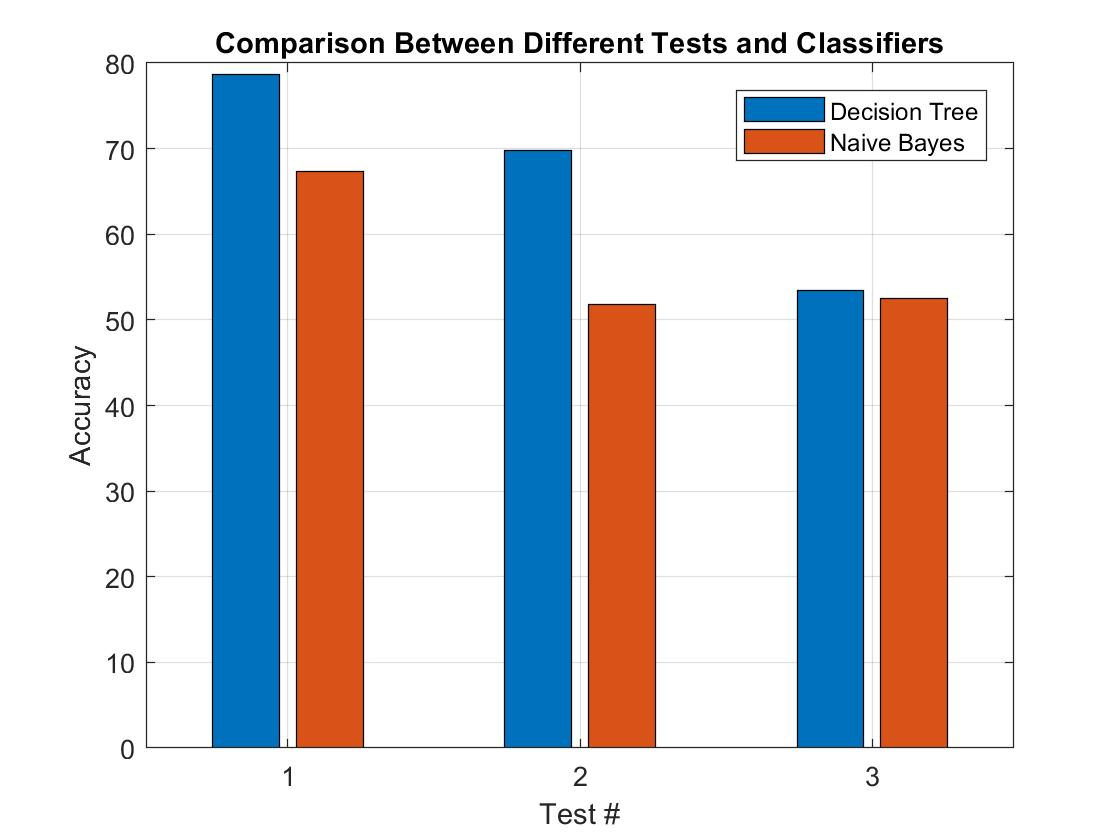
\includegraphics[width = 0.45\textwidth]{comparison.jpg}
        \caption{Accuracy Comparison}
        \label{fig:1}
    \end{figure}
    From the graph Figure 1, we can see that generally, decision tree algorithm has a better overall result comparing to naive Bayes
    classifier. This is reasonable since that we could consider how iTunes Store divides all the artists into categories. And we will 
    use decision tree processes to look for the certain artist. \\
    And for the 3-rd test - genre classification, decision tree algorithm and naive Bayes classifier have kind of the same performance,
    which is also understandable since when we distinguish one genre from another, we will use not only categories but also some "true-false"
    to classify genre.
    %----------------------------------------------------------------------------------------
    %	APPENDIX
    %----------------------------------------------------------------------------------------

    \mbox{~}
    \clearpage
    \begin{appendices}
    \setboolean{@twoside}{false}
    \setboolean{@twocolumn}{false}
        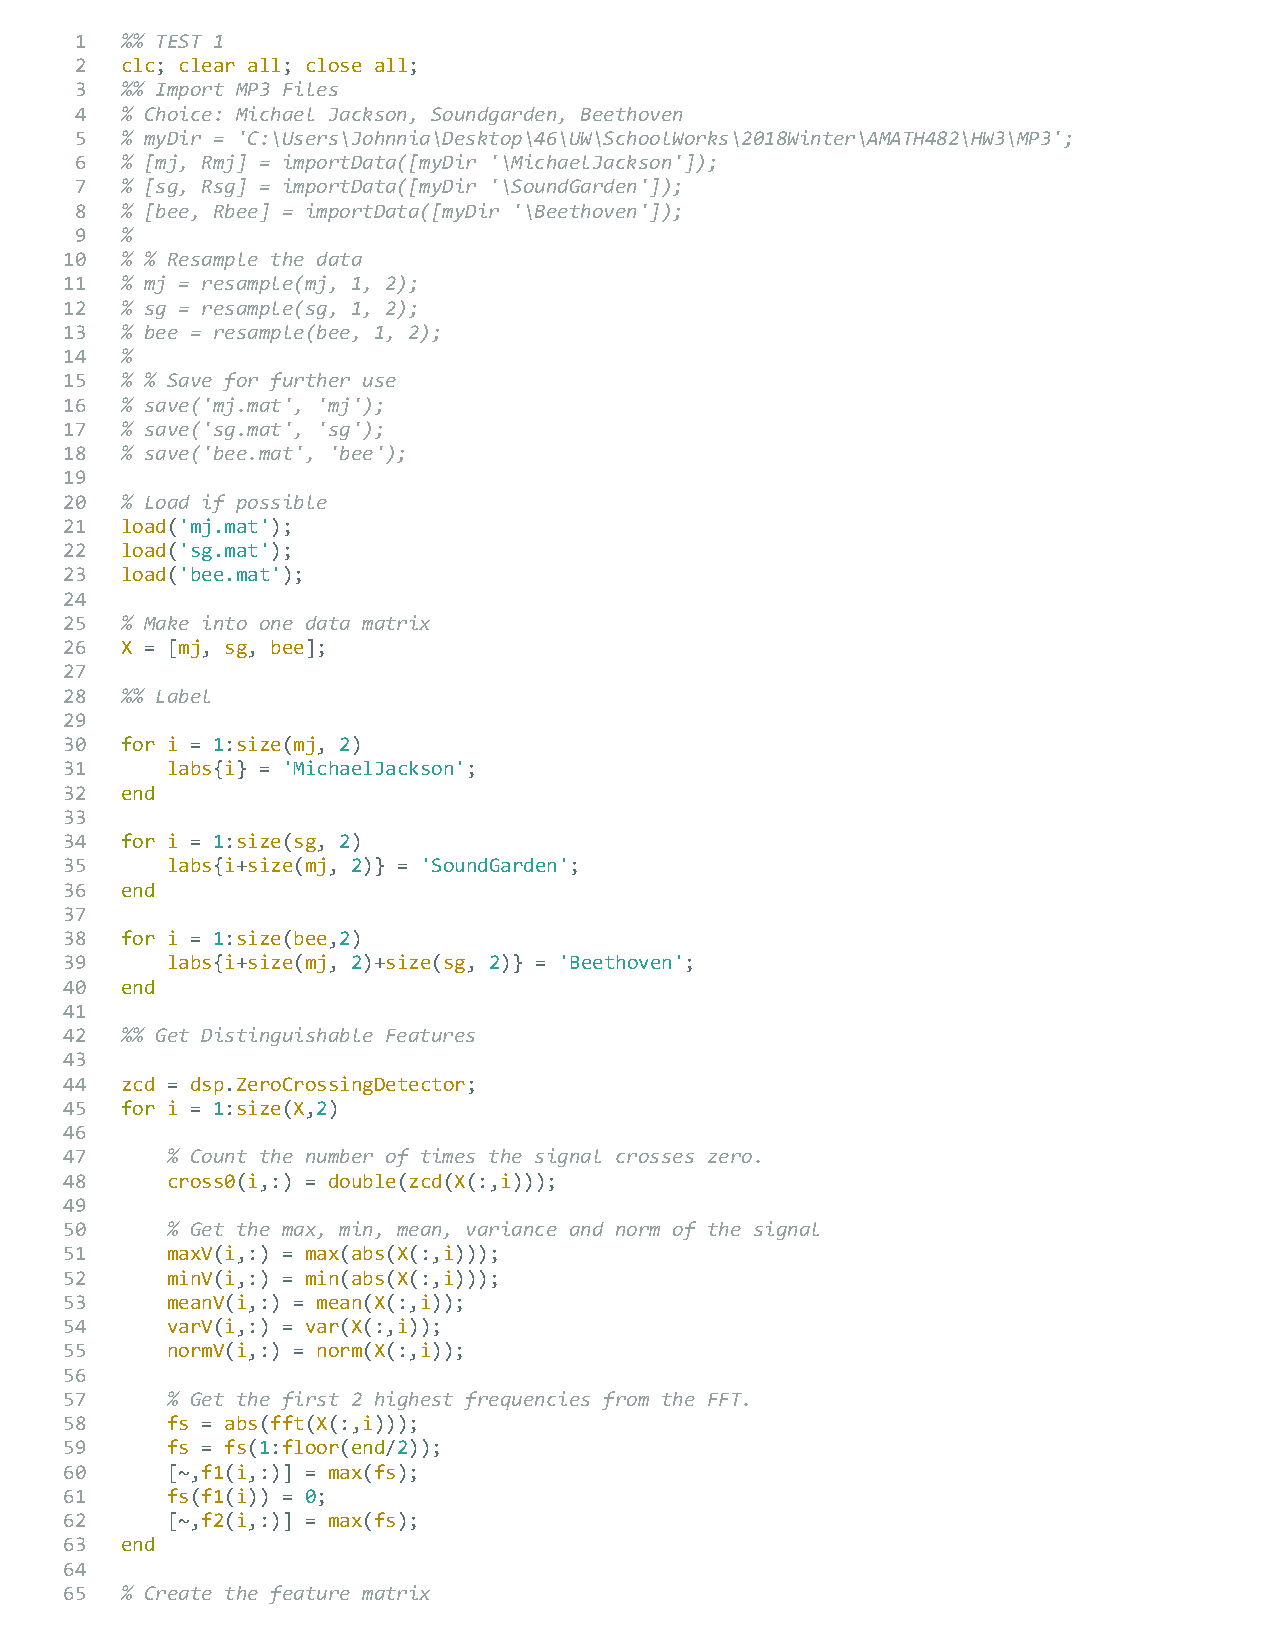
\includepdf[pages=-]{appendix.pdf}
    \end{appendices}

\end{document}